\documentclass[12pt,francais]{report}

\usepackage[UTF8]{inputenc}
\usepackage[pdftex]{graphicx}
\usepackage[french]{babel}
\usepackage{enumitem}
\usepackage{scrextend}
\usepackage{float} 

\begin{document}

\begin{center}

\includegraphics[scale=0.3]{./images/logo_universite_orleans.png}~\\[1.5cm]

\textsc{\large Master 1 - TER}\\[1cm]	

\rule{\linewidth}{0.5mm}\\[0.4cm]

{ \LARGE \bfseries GoodLua\\[0.4cm] }

\rule{\linewidth}{0.5mm}\\[2cm]
\end{center}


\begin{minipage}{0.4\textwidth}
      \begin{flushleft}
			\textsc{Bovie} Pierre-Edouard\\
			\textsc{Labourbe} Loïc\\
			\textsc{Maslowski} Antoine\\
			\textsc{Roche} Julie\\
			\end{flushleft}
    \end{minipage}\hfill
    \begin{minipage}{0.6\textwidth}
      \begin{flushright}
			Enseignants : \textsc{Couvreur} Jean-Michel\\
			\textsc{Dabrowski} Frederic\\

\end{flushright}
    \end{minipage}\\[1.5cm]
		
		\begin{center}
    {7 Février 2018 - 25 Mai 2018}
		\end{center}
	
\chapter*{Partie documentaire}	

\section*{Résumé du projet}	

L’objet du projet est la conception d'un système pour la création et le lancement à distance de programme Lua s'exécutant sur un robot. Le système matériel est composé d'une tablette Androïd et d'un robot mobile à base pcDuino équipé de divers capteurs. Le logiciel de la tablette offrira la possibilité : 
\begin{itemize}
\item de concevoir des programmes
\item de charger à distance le programme sur le robot 
\item de télécommander le robot 
\end{itemize} 
Le système logiciel sur le robot permettra de recevoir et d'exécuter les programmes Lua transmis par la tablette.
		
\newpage 
\section*{Introduction au domaine}

\paragraph*{Quelles sont les possibilités de Blockly ?\\}

Blockly a principalement deux utilités. La première est l'apprentissage de la programmation via un moyen visuel, et la seconde est le développement de programmes embarqués, notamment en robotique.
	
La simplicité d'utilisation de Blockly en fait un outils d'apprentissage très pratique, et ce dès le plus jeune âge. En effet, il suffit de choisir puis glisser des blocs, afin de les imbriquer, comme des pièces de puzzle. Plusieurs sites, jeux et applications proposent des moyens ludiques basés sur Blockly pour apprendre à programmer. Le site le plus connu est celui proposant la série des 'Blockly Games' \cite{ref12}. Existant dans un très grand nombre de langues, il contient plusieurs jeux, de 10 niveaux chacun, avec une augmentation progressive de la difficulté de niveau en niveau et de jeu en jeu afin de découvrir le développement. Le premier de ces jeux est un simple puzzle sur les animaux, afin de découvrir le fonctionnement de Blockly. Le second jeu est un labyrinthe qui utilise des conditionnelles et des boucles. Le jeu suivant, qui permet de diriger les déplacements d'un oiseau, rentre plus sérieusement dans les 2 thèmes du jeu précédent. Suit un jeu qui fait découvrir le dessin via la programmation, puis un autre qui permet de créer des animations évoluant selon le temps. Enfin, on est amenés à coder un petit jeu de tir, tout d'abord avec des blocs, puis en JavaScript à partir de ces blocs. Il existe plusieurs autres séries de jeux basés sur Blockly, on peut notament citer 'Rapid Router' \cite{ref13} qui en 100 niveaux initie les enfants au Python. Ces jeux, généralement accessibles à partir de 8 ans, sont une solution ludique, permise par Blockly pour initier les plus jeunes à la programmation.

Blockly est également utilisé en robotique, dans de nombreux projets. En effet, la bibliothèque étant libre, elle permet de coder ses propres blocs. Les utilisateurs de robots peuvent donc pré-coder les différentes fonctionnalités, et n'ont donc plus qu'à les assembler dans la séquence souhaitée lors de l'exécution. Encore une fois, cette manière d'utiliser Blockly, bien que pratique pour faire du développement embarqué, est aussi et surtout un moyen d'apprendre simplement la programmation sur robot. Par exemple, le robot 'Thymio' \cite{ref14} est un petit robot qui permet de découvrir l'univers de la robotique et sa programmation. Ce robot fournit une intégration de Blockly, qui permet \textit{"de le programmer de façon purement événementielle"}. Un environnement 'Blockly4Thymio' \cite{ref15} a également été ajouté au projet, et offre un apprentissage ludique, destiné à un jeune public.

A l'exception de quelques jeux, généralement mobiles, destinés au grand public et basés sur la librairie Blockly, sa principale utilisation reste donc dans un but éducatif, comme l'avait prévu Google en la créant.


\paragraph*{Quels sont les autres moyens visuels d'apprentissage de la programmation ?\\}

De nos jours de nombreux langages sont développés dans le but de pouvoir enseigner à programmer. Ces langages ont tous des particularités qui permettent de faciliter l'utilisation par des personnes qui sont peu familières avec le monde du développement et peuvent être classées selon deux grandes catégories.

La première regroupe des langages disposant de syntaxes simples ce qui permet une utilisation simple due au fait que l'on traduit d'une manière naturelle ce que l'on attend de notre programme en un code. De plus ces langages sont également utilisés pour développer de réels projets, ce qui permet d'apprendre avec un langage simple mais qui peut être utilisé dans le domaine professionnel. Des exemples pour ces types de langage sont : Python, Ruby.

Le deuxième groupe rassemble des langages visant plus à apprendre le concept de comment programmer plutôt que de réellement apprendre un langage de développement. Pour cela il se base sur une interface graphique simple d'utilisation, le plus généralement les fonctions, actions et événements ont la forme de bloc  que l'utilisateur combinent les un avec les autres en les faisant glisser. Cette catégorie comprend des langages telle que 'Scratch' \cite{ref17}, qui est actuellement utilisé dans les écoles et collèges, 'Alice' \cite{ref19} et 'LEGO Mindstorm Robotics' \cite{ref18}. Ce dernier est d'ailleurs utilisé dans le but d'enseigner le développement pour la robotique car il  permet de programmer des robot tout en restant simple d'utilisation.

\textit{"Most jobs in the future will most likely have some sort of connection to coding"}  Navdeep Bains, Ministre canadien de l'innovation,des science et du dévelopement econimique.

\textit{“ICT used to focus purely on computer literacy – teaching pupils, over and over again, how to word-process, how to work a spreadsheet, how to use programs already creaking into obsolescence; about as much use as teaching children to send a telex or travel in a zeppelin.
Our new curriculum teaches children computer science, information technology and digital literacy: teaching them how to code,and how to create their own programs; not just how to work a computer, but how a computer works and how to make it work for you.”}
Michael Goove, secrétaire d'état a l'éducation du Royaume-Uni (2010-2014) \cite{ref16}

\paragraph*{Comment apprendre à développer grâce à des robots ?\\}

Des personnes ou des sociétés de plusieurs horizons ont cherché à rendre accessible l'apprentissage de la programmation via des robots, en voici quelques exemples :

Jacqueline M. Kory Westlund est une chercheuse travaillant au MIT. Son domaine de recherche est les interactions entre l'homme et la machine.
Elle crée des robots pour les enfants et étudie leurs relations et les possibilités d'apprentissage.\cite{ref9}
Le robot est dirigé par une application sous Android.

'Cozmo' est un robot développé par la société Anki. Ce robot possède la technologie 'Code Lab', qui est basée sur Scratch.\cite{ref10} 
'Code Lab' possède une interface graphique intuitive et propose une manière simple de programmer le robot.
Chaque fonctionnalité est représentée par un bloc d'une certaine forme.
Ces blocs s'assemblent les uns dans les autres et permettent à un utilisateur sans connaissance en programmation d'ajouter une nouvelle fonctionnalité au robot.

'Hexa' est un robot produit par la société Vincross. Devant l'absence d'OS orienté robot, ils ont créé le leur: 'MIND' \cite{ref11},
basé sur une architecture Linux. De nombreuses librairies sont proposées afin de contrôler facilement le robot.
Une de leurs librairies propose une interface 3D afin de permettre aux non-développeurs de créer des mouvements et des comportements complexes.
Une application est disponible sur iOS et android pour contrôler le robot à distance.

\paragraph*{Quelles sont les possibilités de l'embarqué ?\\}

La programmation embarquée est un vaste domaine, allant des systèmes embarqués de voitures à tous les objets connectés de la maison, et est décomposable en de nombreux sous-domaines. Nous allons ici plus particulièrement nous intéresser aux possibilités offertes par l'arduino en matière d'embarqué.

La domotique est l'un des champs d'utilisation d'un arduino \cite{ref20}. Grâce à leur petite taille, beaucoup d'objets domestiques sont contrôlés par des arduinos. Prenons par exemples quelques objets que l'on peut utiliser dans son jardin, et qu'il est possible de créer soi-même, ou qui existent dans le commerce, et qui utilisent un arduino \cite{ref21}: 

- un verrou électrique à code, pour sécuriser un portail, contrôlé par un arduino, et composé d'un verrou, d'un clavier et d'un afficheur LED, auquel on peut aussi ajouter un lecteur de badges RDID (identification par radiofréquence).

- un arrosage automatique, composé d'une sonde de détection d'humidité, une vanne électromagnétique, et une carte arduino, qui selon le niveau d'humidité du sol va activer un arrosage.

- un lampadaire, qui grâce à un capteur de lumière et un arduino pourra s'allumer de la tombée de la nuit jusqu'à une certaine heure.

- une station météo, qui pourra surveiller la luminosité, la température et l'humidité, et vous prévenir sur votre smartphone.

Arduino est également beaucoup utilisé en robotique, car ces cartes permettent de contrôler plusieurs éléments, d'autant plus lorsqu'elles sont associées à un micro-ordinateur (Raspberry Pi, pcDuino). Par exemple, une carte pourra contrôler l'activation des moteurs, tout en surveillant leur chaleur grâce à un capteur, et les arrêter en cas de surchauffe. Elle pourra aussi recevoir des informations transmises par des capteurs infrarouges, ultrasons, ou même une caméra, et réagir en conséquence. \cite{ref22}

Les champs des utilisations d'arduino étant très vaste, l'imagination de sa communauté d'utilisateurs en est la seule limite. Parmis les projets sortant de l'ordinaire, ont été créés un fauteuil roulant motorisé avec joystick \cite{ref23}, des jouets tels que des petits trains autonomes ou des voitures télécommandées, un gps, des volets roulants connectés, un incubateur d'oeufs connecté \cite{ref24}, et bien d'autres.


\newpage
\section*{Analyse de l'existant}

Nous avons reçu pour ce projet, un kit matériel qui forme le robot.\\
Pour nous aider à découvrir son utilisation, nous avons étudié le projet d'algorithmique répartie des étudiants de la promotion 2015 des master 1 informatique \cite{ref1} dans lequel ils manipulent un robot semblable au notre, mais avec des des langages différent du notre (eLua) puisqu'ils l'ont contrôlé avec du python et du C++.

\begin{figure}[!h]
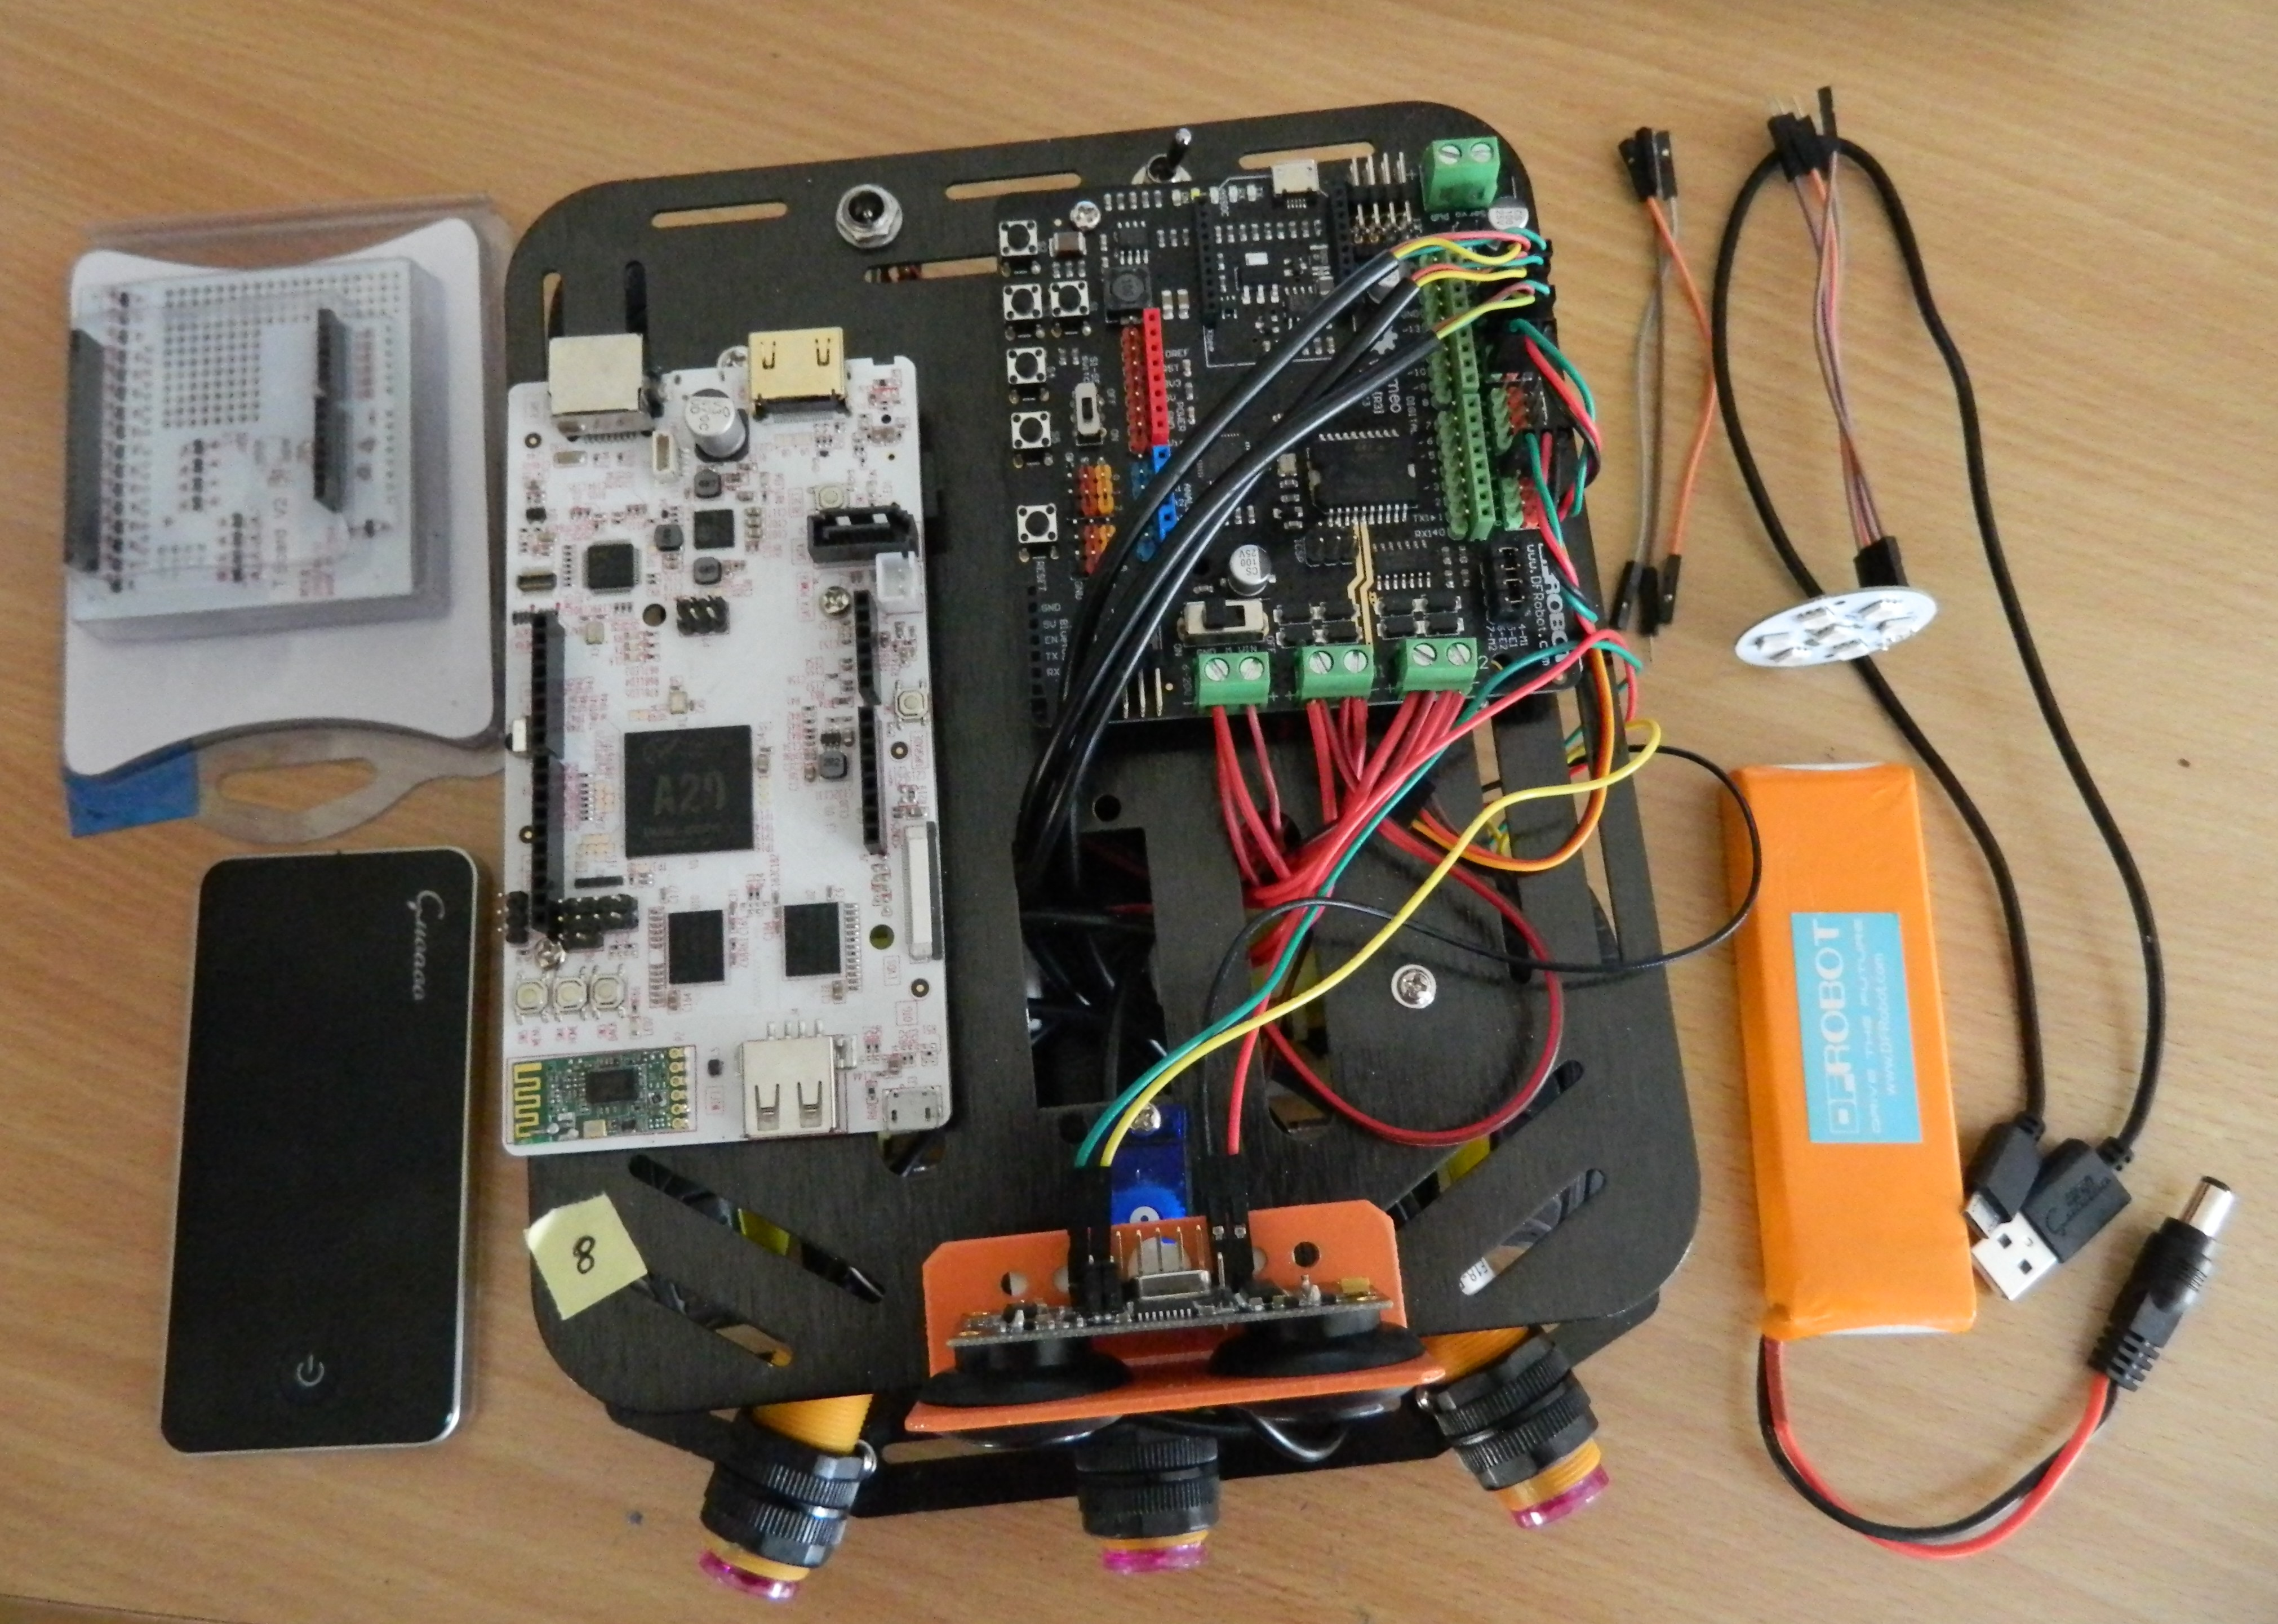
\includegraphics[scale=0.4]{./images/notre_materiel.jpg}~\
\caption{Notre materiel}
\end{figure}
	
Voici la liste du matériel dont nous disposons et dont nous devrons nous servir pour ce projet :

\begin{description}
\item [Le pcDuino :] La carte pcDuino V3 est un mini PC possédant un processeur dual core A20. Une fois branchée à un écran, un clavier et une souris, grâce à son port USB, elle s'utilise de la même manière qu'un PC sous une distribution Ubuntu. Elle possède un lecteur de carte micro-sd,  c'est dans cette carte que se situe le système d'exploitation du pcDuino. Le pcDuino possède également un port ethernet ainsi qu'une carte wifi, ce qui permet de se connecter à un réseau facilement. Pour le faire fonctionner, il suffit de le brancher à un chargeur USB par son port micro USB. Il possède enfin des broches arduino, en plus de ses interfaces de communication, permettant de faire de la programmation arduino.\cite{ref3}
\item [L'arduino :] L'arduino Romeo V2.2 (R3) \cite{ref4} est un micro-contrôleur tout en un spécialement créé pour la robotique, qui fournit des interfaces de puissance pour contrôler des moteurs.
\item [La plateforme mobile :] Notre robot est composé d'une châssis Baron - 4WD auquel sont associés 4 moteurs reliés à 4 roues codeuses. \cite{ref5}
\item [La LED :] Le disque contient 7 LEDs RGB \cite{ref6}, que l'ont peut allumer grâce à 3 pins, un pour chaque couleur, ainsi qu'avec un pin d'alimentation.
\item [Les capteurs infrarouges :] Les 3 capteurs possèdent une LED qui s'allume si un objet est dans le champ de détection. Ils ont une sortie binaire, selon si un obstacle est détecté ou non. Leur distance de détection peut être de 3 à 80 cm, et se règle manuellement avant l'utilisation. \cite{ref7}
\item [Le capteur ultrasons :] Lié à l'arduino, il détecte des températures allant de -10 à environ 70 degrés celsius, à une distance de 4cm, jusqu'à 5m. \cite{ref8}
\end{description}

\bigskip
\begin{description}
\item [Blockly :] Nous utilisons la bibliothèque Blockly \cite{ref2} pour avoir un éditeur de code visuel. Blockly se présente sous forme de pièces de puzzle, chacune représentant un concept de code, comme une fonction, une condition, une boucle ou une variable. L'utilisateur n'a donc qu'à sélectionner et faire glisser les pièces pour les placer et les  imbriquer, afin de former un programme. Il n'a donc pas à s'occuper de la syntaxe, puisque les formes des pièces lui indiquent où il peut les placer ou non. Une fois le programme formé, Blockly peut le transformer en différents langages (JavaScript, Python, PHP, Dart) dont celui qui nous intéresse pour ce projet, le Lua.\\
Grâce à cette bibliothèque, nous avons la possibilité de créer les blocs de notre choix, correspondant à des fonctions à appliquer sur le robot, d'intégrer l'éditeur Blockly à notre application Androïd, et de générer le code à exécuter.
\end{description}

\chapter*{Cahier des charges}

\section*{Besoins fonctionnels}

\begin{itemize}[label=\textbullet]
	\item \textbf{Exécuter du code}
	\begin{description}
		\item \textit{description :} exécuter du code eLua sur le PcDuino
		\item \textit{priorité :} très haute
		\item \textit{justification :} cette fonctionnalité est la principale. Nous devons être en mesure de faire fonctionner le robot grâce à du code eLua avant toute autre chose.
		\item \textit{test prévu :} Tet d'exécution simple, l'équivalent du "Hello world" sur pcDuino, c'est à dire l'allumage d'une LED via du code Lua.
	\end{description}
	\item \textbf{Connecter android au robot grâce au wifi}
	\begin{description}
		\item \textit{description :} utiliser la carte wifi du PcDuino pour la connecter à un appareil androïd.
		\item \textit{priorité :} haute
		\item \textit{justification :} le code crée via l'application androïd doit être transmis au robot pour être exécuté. Une solution filaire étant peu pratique, nous le connecterons via wifi.
	\item \textit{test prévu :} Envoi de fichiers et de commandes de la tablette vers le pcDuino, et inversement.
	\end{description}
	\item \textbf{Transformer blockly en eLua}
	\begin{description}
		\item \textit{description :} traduire les blocs de la librairie Blockly dans le langage Lua, plus spécifiquement en eLua.
		\item \textit{priorité :} moyenne
		\item \textit{justification :} le robot étant "guidé" par du code eLua, il est nécessaire de procéder à une traduction du programme visuel dans ce langage avant de l'envoyer au robot pour être exécuté.
	\end{description}
	\item \textbf{Créer un programme}
	\begin{description}
		\item \textit{description :} la création d'un nouveau programme blockly via l'application androïd.
		\item \textit{priorité :} moyenne
		\item \textit{justification :} c'est la fonctionnalité de base de l'application, il faut pouvoir créer de nouveaux programmes en vue de les écrire et de les exécuter.
	\end{description}
	\item \textbf{Sauvegarder / Charger des programmes}
	\begin{description}
		\item \textit{description :} l'utilisateur pourra sauvegarder les programmes sur lesquels il travaille, et reprendre sa progression là où il était en chargeant un programme parmi ceux enregistrés.
		\item \textit{priorité :} basse
		\item \textit{justification :} cela permettra de travailler sur un programme en plusieurs fois sans risque de perdre son travail. Cette fonctionnalité était à la base en option, mais l'architecture de notre application nécessite de pouvoir l'utiliser.
		\item \textit{test prévu :} Enregistrer un programme traduit en lua dans un fichier sur la tablette.
	\end{description}
\end{itemize}

\bigskip

\section*{Besoins non fonctionnels}

\begin{description}
	\item [Environnement de travail :]Nous travaillons sous une distribution Ubuntu. Pour la partie programmation en eLua, une version embarquée du langage Lua \cite{refLua}, il est possible d'utiliser n'importe quel éditeur de texte, puis de compiler le fichier.
	\item [Exécution en temps réel / rapidité :] Il serait préférable que l'exécution d'un programme se fasse de manière assez rapide, pour ne pas aller contre les attentes de l'utilisateur. Par exemple, si le programme utilise des capteurs, mais qu'une lenteur dans le programme fait qu'un obstacle n'est pas détecté à temps, cela nuira à l'expérience de l'utilisateur. De même, l'un des buts de l'application, est de pouvoir exécuter une séquence, ou de donner des ordres au robot en temps réel. 
	\item [Simplicité d'utilisation : ]L'application doit être utilisable par des utilisateurs sachant programmer, qui pourront créer un programme complexe à partir des blocs basiques, mais elle doit également être accessible à des utilisateurs débutants en programmation, qui pourront utiliser des blocs représentant des fonctions toutes faites concernant le robot (par exemple : allumer LED). Les blocs et l'interface devront donc être instinctifs et simples d'utilisation.
	\item [Empreinte mémoire :] Le poids de l'application Androïd doit être le plus petit possible car la tablette possède une mémoire limitée.
	\item [Empreinte énergétique :] L'application ne doit pas surconsommer la batterie de la tablette, pour cela nous allons contrôler l'utilisation des ressources.
\end{description}

\section*{Prototype - l'interface de l'application Androïd }
En ouvrant l'application, l'utilisateur se verra proposer de créer un nouveau programme, il devra alors lui donner un nom, ou alors de charger un programme déjà existant, en choisissant dans une liste. Une fois le programme sélectionné ou créé, il aura le choix de le modifier ou de l'exécuter. [Figure 1]

Dans le cas du choix de modifier le code, on ouvrira l'éditeur visuel contenant Blockly avec l'ensemble des blocs disponibles dans une barre latérale gauche. Un menu permettra également de sauvegarder le programme en cours d'édition ou de l'effacer. [Figure \ref{figMaquette}]\\

\begin{figure}[!h]
\begin{addmargin}[-7em]{1em}
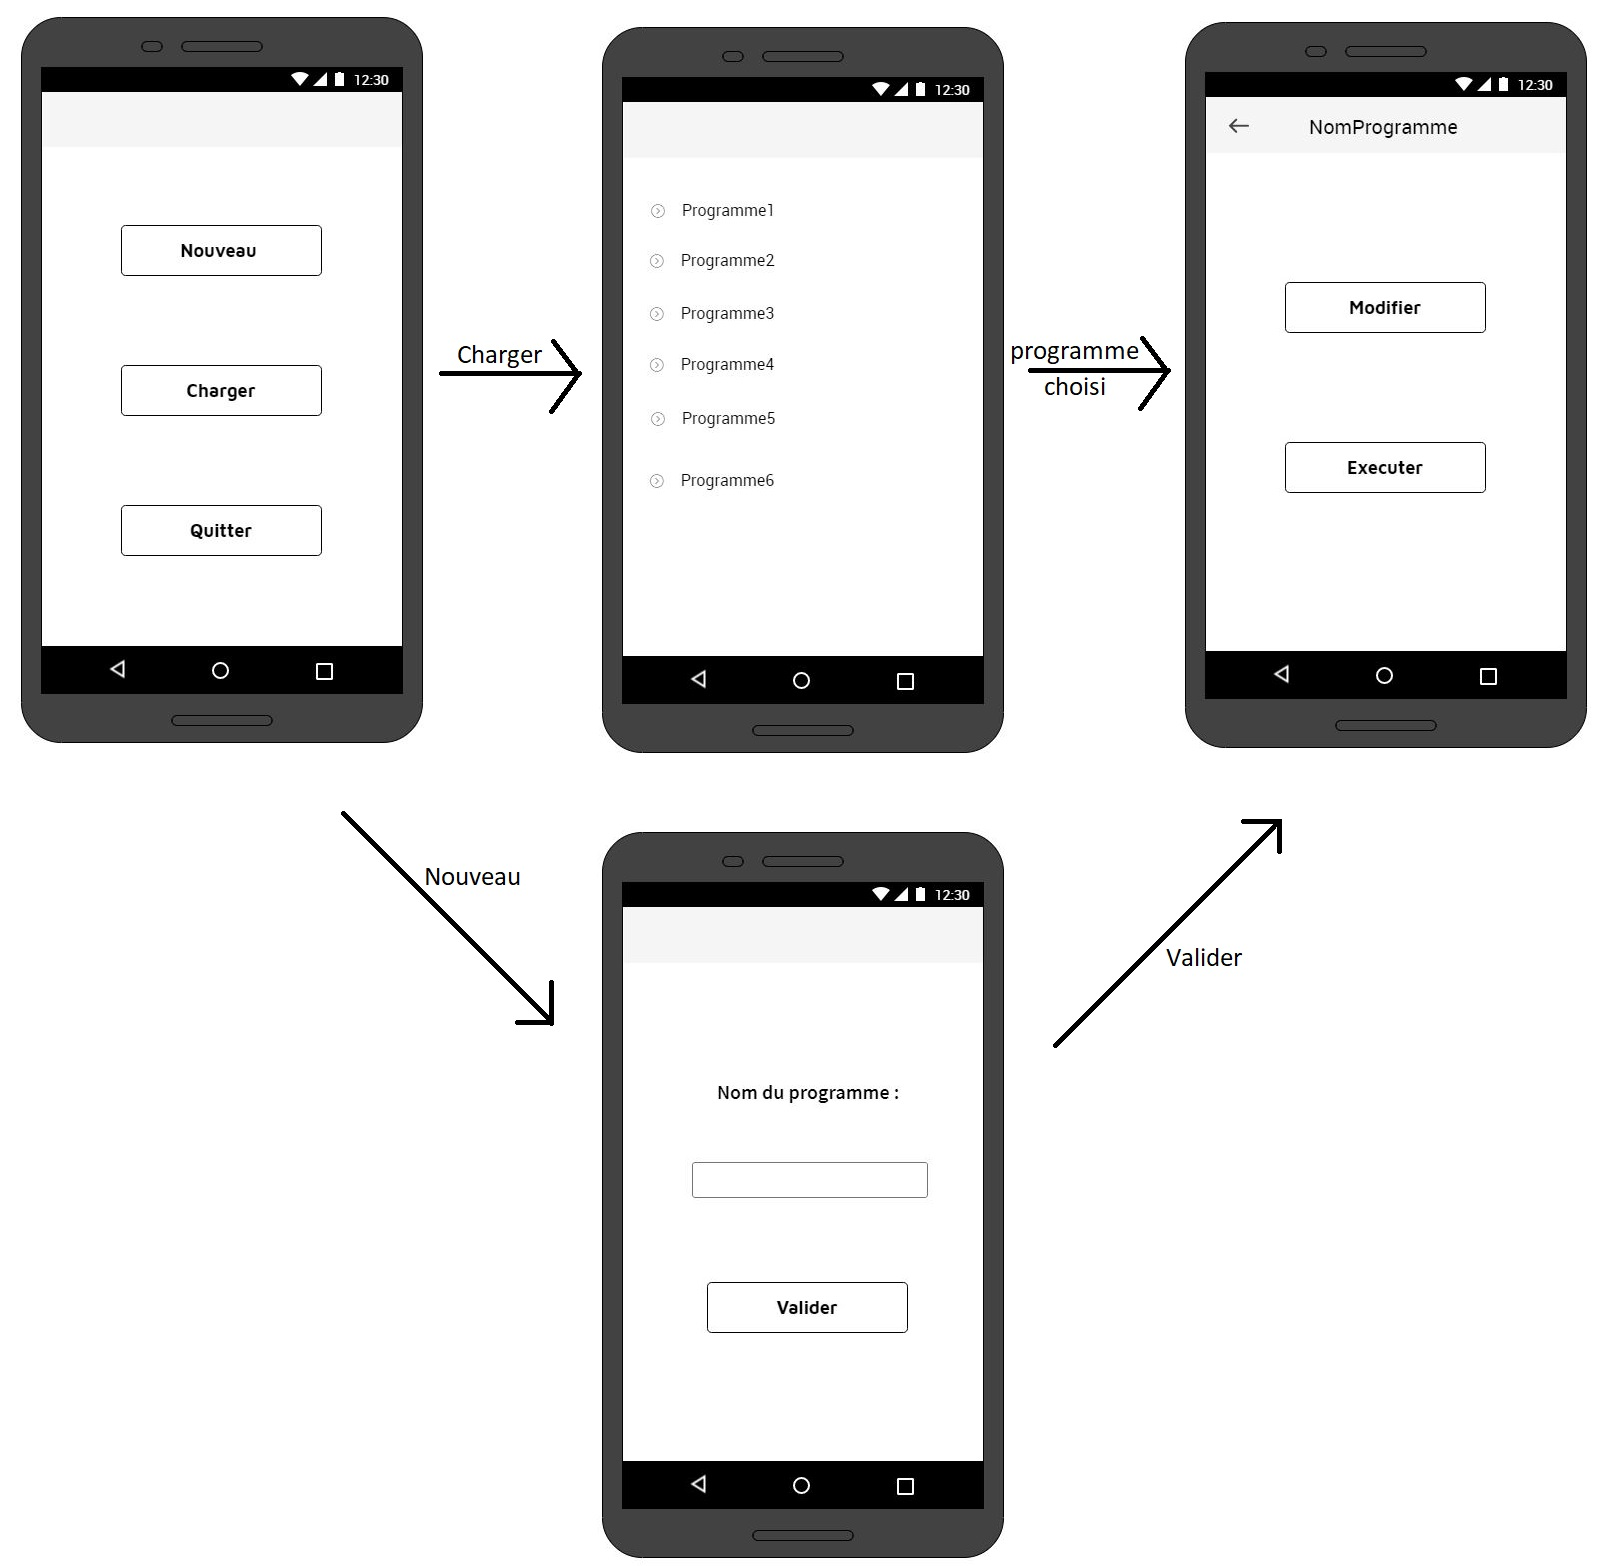
\includegraphics[scale=0.45]{./images/maquette1.jpg}~\\[1.5cm]
\caption{Maquette 1ère partie}
\end{addmargin}
\end{figure}

\begin{figure}[!h]
\begin{addmargin}[-5em]{1em}
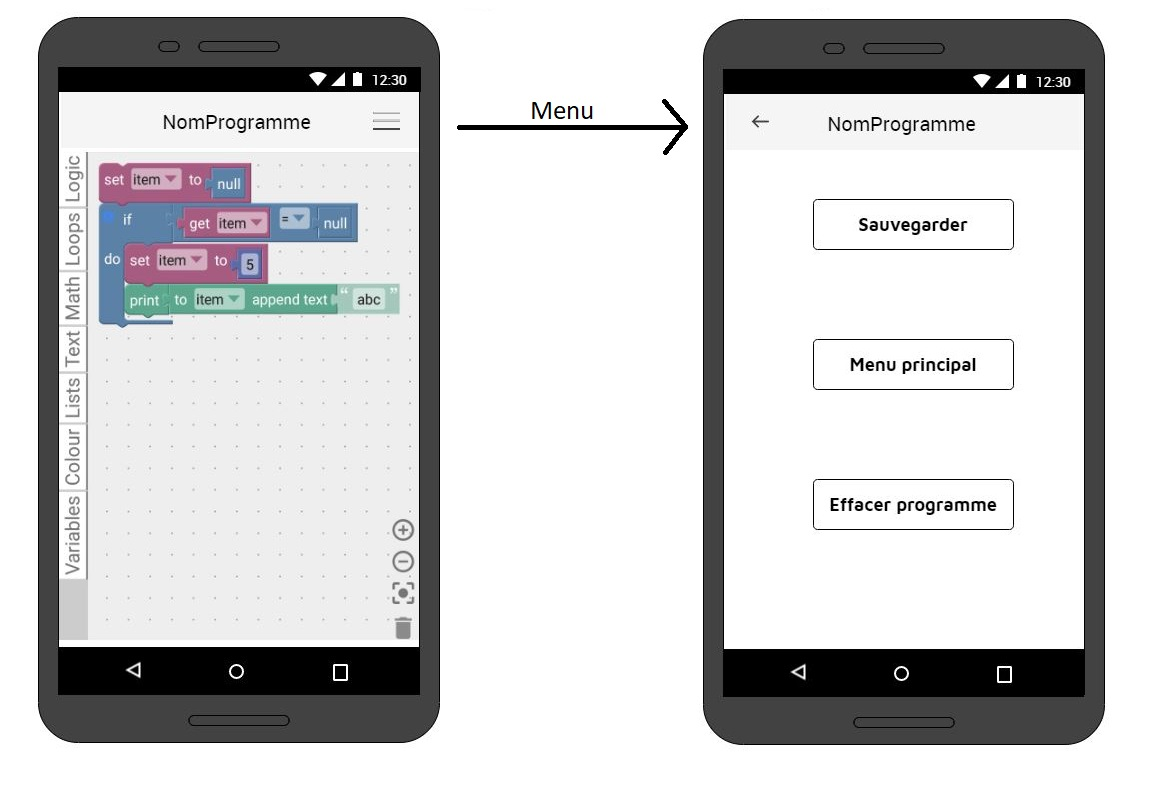
\includegraphics[scale=0.6]{./images/maquette2.jpg}~\\[1.5cm]
\caption{Maquette 2ème partie}
\label{figMaquette}
\end{addmargin}
\end{figure}



\chapter*{Planning}

Planning effectif jusqu'au rendu du présent rapport :\\
\begin{figure}[!h]
\begin{addmargin}[-7em]{1em}
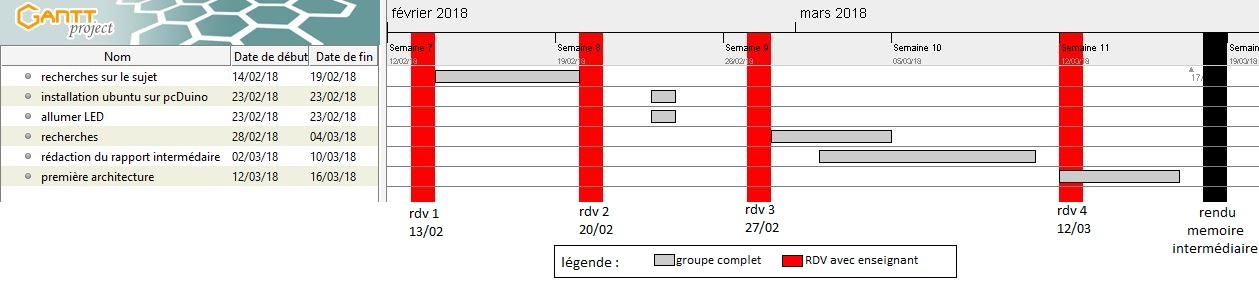
\includegraphics[scale=0.6]{./images/intermediaireEffectif.jpg}~\\[1.5cm]
\caption{Planning du 13 février au 18 mars}
\end{addmargin}
\end{figure}

\newpage
Planning prévisionnel pour la suite du projet :\\
\begin{figure}[!h]
\begin{addmargin}[-8em]{1em}
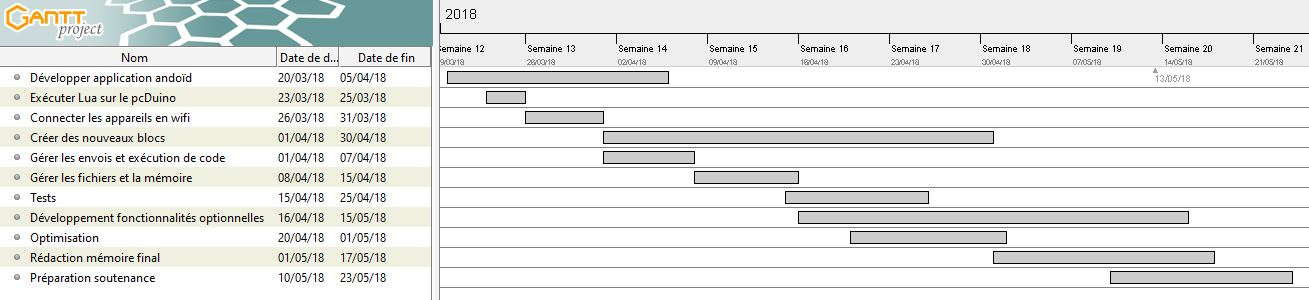
\includegraphics[scale=0.6]{./images/previsionnel.jpg}~\\[1.5cm]
\caption{Planning du 19 mars au 25 mai}
\end{addmargin}
\end{figure}

\textbf{Répartition du travail :}
Durant toute la phase de recherche et de réflexion, nous nous sommes répartis les points sur lesquels il fallait trouver des informations, et nous avons régulièrement rassemblés les connaissances trouvées.
Pour la programmation de l'application et du robot, nous prévoyons de beaucoup travailler ensemble, puisque nous n'avons qu'un robot et une tablette, mais certaines tâches seront réparties, comme par exemple la création des nouveaux blocs Blockly propre à notre projet, certaines fonctionnalités de l'application testables via Android Studio, ou l'écriture des tests unitaires. En revanche des tâches comme la connexion du robot à la tablette, l'écriture du code Lua ou les tests sur le matériel ne pourront être réalisés qu'avec le groupe complet.


\bibliographystyle{unsrt}
\bibliography{biblio}

\end{document}
